  \subsection{Medición de la tensión eficaz de una onda proveniente de un circuito de control de ángulo de conducción}
Para la siguiente parte del experimento, se utiliza un circuito de medición 
de ángulo de disparo. El mismo se enseña en la Figura \ref{fig:CircuitoTriac}.

\begin{figure}[H]
  \centering
  \frame{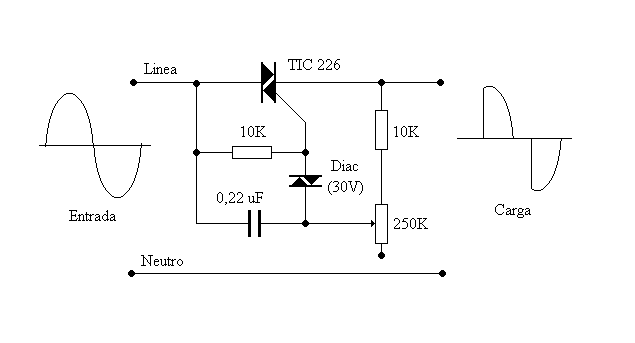
\includegraphics[width=0.6\textwidth]{Imagenes/ActividadPractica/MedicionDeTensionEficazConCircuitoTriac/Esquema_Circuito_Angulo_Disparo.png}}
  \caption{Esquema del circuito de control de ángulo de disparo.}
  \label{fig:CircuitoTriac}
\end{figure}

El procedimiento consiste en medir la tensión de entrada al circuito, 
y medir la de salida sobre la carga, tomando lecturas
al variar el ángulo de conducción con un multímetro que mide True RMS y otro de valor medio. 
Luego se debe confeccionar un gráfico normalizado de tension de salida 
respecto de la entrada, con las curvas obtenidas con cada instrumento.

El esquema de conexión se presenta a continuación en la Figura \ref{fig:EsquemaConexionTriac}.

\begin{figure}[H]
  \centering
  \frame{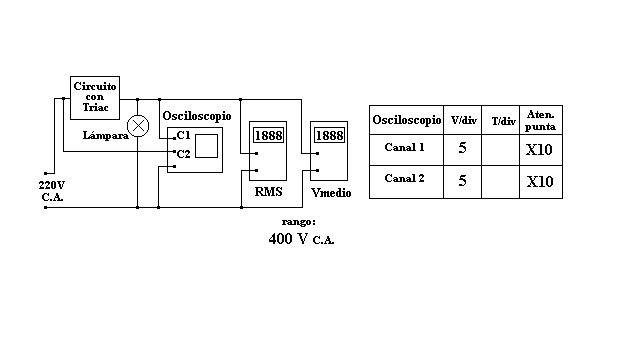
\includegraphics[width=0.5\textwidth]{Imagenes/ActividadPractica/MedicionDeTensionEficazConCircuitoTriac/Esquema_Conexion_Circuito_Angulo_Disparo.png}}
  \caption{Esquema de conexión para el relevamiento de curva.}
  \label{fig:EsquemaConexionTriac}
\end{figure}

Se presentan a continuación los valores tabulados.

\begin{table}[H]
\centering
  \begin{tabular}{|c|c|c|c|c|}
    \hline
      Fase & $Vo_1$[V] & $Vo_2$[V] & $(\frac{Vo_1}{V_{in}})$[V] & Bla $(\frac{Vo_2}{V_{in}})$[V] \\
    \hline
      0°    & 234     & 234     & 1,064   & 1,064\\
      36°   & 222,8   & 211,6   & 1,013   & 0,962\\
      72°   & 194,5   & 158,6   & 0,884   & 0,721\\
      108°  & 135,8   & 189,6   & 0,617   & 0,407\\
      144°  & 58,77   & 30,0    & 0,267   & 0,136\\
      180°  & 0       & 0       & 0       & 0\\
    \hline
  \end{tabular}
\end{table}



